\documentclass{article}
\usepackage[utf8]{inputenc}
\usepackage[super,square]{natbib}
\usepackage{tabularx}
\usepackage{parskip}
\usepackage[margin=1.4in]{geometry}
\usepackage{csquotes}
\usepackage{amsmath}
\usepackage{amsfonts}
\usepackage{amsthm}
\usepackage{hyperref}
\usepackage{graphicx}
\usepackage{float}

\newcommand{\comment}[1]{}

\title{\vspace{-3cm} Object-Oriented Programming and Design Patterns}
\author{}
\date{}


\comment{
TODO:
- simplify OOD section by using defintions in appendix and remove unnecessary elaborations
- add application and consequence section to starred patterns
}
\begin{document}
\maketitle
\vspace{-1.5cm}
\tableofcontents
\newpage
\section{Object-Oriented Design}
\subsection{Classes, Objects and Interfaces}

Object-oriented programs are made up of \textbf{objects}. An object packages both data and the procedures that operate on that data. The procedures are typically called \textbf{methods} or \textbf{operations}. An object performs an operation when it receives a request (or message) from a client.

\textbf{Requests} are the only way to get an object to execute an operation. Operations are the only way to change an object's internal data. Because of these restrictions, the object's internal state is said to be \textbf{encapsulated}; it cannot be accessed directly, and its representation is invisible from outside the object.

Every operation declared by an object specifies the operation's name, the objects it takes as parameters, and the operation's return value. This is known as the operation's \textbf{signature}. The set of all signatures defined by an object's operations is called the \textbf{interface} to the object. An object's interface characterizes the complete set of requests that can be sent to the object. Any request that matches a signature in the object's interface may be sent to the object.

A \textbf{type} is a name used to denote a particular interface. An object may have many types, and widely different objects can share a type. The class defines the object's internal state and the implementation of its operations. In contrast, an object's type only refers to its interface — the set of requests to which it can respond. Part of an object's interface may be characterized by one type, and other parts by other types. Two objects of the same type need only share parts of their interfaces. Interfaces can contain other interfaces as subsets. We say that a type is a subtype of another if its interface contains the interface of its supertype. Often we speak of a subtype inheriting the interface of its supertype.

Objects are created by instantiating a \textbf{class}. The object is said to be an \textbf{instance} of the class. The process of instantiating a class allocates storage for the object's internal data (made up of instance variables) and associates the operations with these data. Many similar instances of an object can be created by instantiating a class.

A useful analogy is as follows: A blueprint for a house design is like a class description. All the houses built from that blueprint are objects of that class. A given house is an instance.

\subsection{Polymorphism}

The run-time association of a request to an object and one of its operations is known as \textbf{dynamic binding}, which means that issuing a request doesn't commit you to a particular implementation until run-time. Consequently, you can write programs that expect an object with a particular interface, knowing that any object that has the correct interface will accept the request. Moreover, dynamic binding lets you substitute objects that have identical interfaces for each other at run-time. This substitutability is known as \textbf{polymorphism}, and it's a key concept in object-oriented systems. It lets a client object make few assumptions about other objects beyond supporting a particular interface. Polymorphism simplifies the definitions of clients, decouples objects from each other, and lets them vary their relationships to each other at run-time.

\subsection{Inheritence}

New classes can be defined in terms of existing classes using class \textbf{inheritance}. Class inheritance is basically just a mechanism for extending an application's functionality by reusing functionality in parent classes. When a subclass inherits from a parent class, it includes the definitions of all the data and operations that the parent class defines. Objects that are instances of the subclass will contain all data defined by the subclass and its parent classes, and they'll be able to perform all operations defined by this subclass and its parents. Inheritance's ability to define
families of objects with identical interfaces (usually by inheriting from an abstract class) is what allows polymorphism to work. 

Implementation dependencies can cause problems when you're trying to reuse a subclass. Should any aspect of the inherited implementation not be appropriate for new problem domains, the parent class must be rewritten or replaced by something more appropriate. This dependency limits flexibility and ultimately reusability. One cure for this is to inherit only from abstract classes, since they usually provide little or no implementation.

An \textbf{abstract class} is one whose main purpose is to define a common interface for its subclasses. An abstract class will defer some or all of its implementation to operations defined in subclasses; hence an abstract class cannot be instantiated. The operations that an abstract class declares but doesn't implement are called abstract operations. Classes that aren't abstract are called \textbf{concrete classes}.

Subclasses can refine and redefine behaviors of their parent classes. More specifically, a class may override an operation defined by its parent class. \textbf{Overriding} gives subclasses a chance to handle requests instead of their parent classes. 

Class inheritance lets you define classes simply by extending other classes, making it easy to define families of objects having related functionality. In contrast to class inheritance, interface inheritance or \textbf{subtyping} describes when an object can be used in place of another.

A \textbf{mixin class} is a class that's intended to provide an optional interface or methods to other classes without having to be the parent class of those other classes. It's similar to an abstract class in that it's not intended to be instantiated. Mixin classes require multiple inheritance.

\subsection{Interfaces}

\textbf{Program to an interface, not an implementation}

This principle of object-oriented design has two main benefits:
\begin{enumerate}
    \item Clients remain unaware of the specific types of objects they use, as long as the objects adhere to the interface that clients expect.
    \item Clients remain unaware of the classes that implement these objects. Clients only know about the abstract classes defining the interface.    This greatly reduces implementation dependencies between subsystems
\end{enumerate}

Don't declare variables to be instances of particular concrete classes. Instead, commit only to an interface defined by an abstract class. Though you will need to instantiate concrete classes in order to specify a particular implementation somewhere in your system -- the creational patterns ensure that your system is written in terms of interfaces, not implementations.

\subsection{Composition}

\textbf{Favor object composition over class inheritance.}

The two most common techniques for reusing functionality in object-oriented systems are class inheritance and object composition. Reuse by subclassing is often referred to as \textbf{white-box reuse}. The term ``white-box" refers to visibility: With inheritance, the internals of parent classes are often visible to subclasses.

Object composition is an alternative to class inheritance. Here, new functionality is obtained by assembling or composing objects to get more complex functionality. Object composition requires that the objects being composed have well-defined interfaces. This style of reuse is called \textbf{black-box reuse}, because no internal details of objects are visible. Objects appear only as ``black boxes."

Because objects are accessed solely through their interfaces, we don't break encapsulation. Any object can be replaced at run-time by another as long as it has the same type. Moreover, because an object's implementation will be written in terms of object interfaces, there are substantially fewer implementation dependencies.

Additionally, favoring object composition over class inheritance helps you keep each class encapsulated and focused on one task. Your classes and class hierarchies will remain small and will be less likely to grow into unmanageable monsters. On the other hand, a design based on object composition will have more objects (if fewer classes), and the system's behavior will depend on their inter relationships instead of being defined in one class.

\subsection{Delegation}
Delegation is a way of making composition as powerful for reuse as inheritance. In delegation, two objects are involved in handling a request: a receiving object delegates operations to its delegate. This is analogous to subclasses deferring requests to parent classes. Delegation is an extreme example of object composition. It shows that you can always replace inheritance with object composition as a mechanism for code reuse.

For example, instead of making class Window a subclass of Rectangle (because windows happen to be rectangular), the Window class might reuse the behavior of Rectangle by keeping a Rectangle instance variable and delegating Rectangle-specific behavior to it. In other words, instead of a Window being a Rectangle, it would have a Rectangle and may call the Area method.

The main advantage of delegation is that it makes it easy to compose behaviors at run-time and to change the way they're composed. Our window can become circular at run-time simply by replacing its Rectangle instance with a Circle instance, assuming Rectangle and Circle have the same type.

Delegation has a disadvantage it shares with other techniques that make software more flexible through object composition: Dynamic, highly parameterized software is harder to understand than more static software.There are also run-time inefficiencies, but the human inefficiencies are more important in the long run. Delegation is a good design choice only when it simplifies more than it complicates.

\subsection{Parameterized Types}
Parameterized types give us a third way (in addition to class inheritance and object composition) to compose behavior in object-oriented systems. This
technique lets you define a type without specifying all the other types it uses. The unspecified types are supplied as parameters at the point of use. For example, a List class is parameterized by the type of elements it contains.


\subsection{Run-Time and Compile-Time Structures}

Object composition lets you change the behavior being composed at run-time, but it also requires indirection and can be less efficient. Inheritance lets you provide default implementations for operations and lets subclasses override them. Parameterized types let you change the types that a class can use. But neither inheritance nor parameterized types can change at run-time.

Many design patterns (in particular those that have object scope) capture the distinction between compile-time and run-time structures explicitly. Composite and Decorator patterns are especially useful for building complex run-time structures. Observer involves run-time structures that are often hard to understand unless you know the pattern. Chain of Responsibility also results in communication patterns that inheritance doesn't reveal. In general, the run-time structures aren't clear from the code until you understand the patterns.

\newpage
\section{Design Patterns}

We classify design patterns by two criteria. The first criterion, called \textbf{purpose}, reflects what a pattern does. Patterns can have either \textbf{creational}, \textbf{structural}, or \textbf{behavioral} purpose. Creational patterns concern the process of object creation. Structural patterns deal with the composition of classes or objects. Behavioral patterns characterize the ways in which classes or objects interact and distribute responsibility.

The second criterion, called \textbf{scope}, specifies whether the pattern applies primarily to classes or to objects. Class patterns deal with relationships between classes and their subclasses. These relationships are established through inheritance, so they are static — fixed at compile-time. Object patterns deal with object relationships, which can be changed at run-time and are more dynamic. Almost all patterns use inheritance to some extent. So the only patterns labeled ``class patterns" are those that focus on class relationships. Note that most patterns are in the Object scope.

Creational class patterns defer some part of object creation to subclasses, while Creational object patterns defer it to another object. The Structural class patterns use inheritance to compose classes, while the Structural object patterns describe ways to assemble objects. The Behavioral class patterns use inheritance to describe algorithms and flow of control, whereas the Behavioral object patterns describe how a group of objects cooperate to perform a task that no single object can carry out alone

Each design pattern lets some aspect of a system's structure vary independently of other aspects, thereby making a system more robust to a particular kind of change.

\begin{enumerate}
    \item \textbf{Creating an object by specifying a class explicitly}
    
    Avoid with: Abstract Factory, Factory Method, Prototype. 
    
    \item \textbf{Dependence on specific operations.}
    
    Avoid with: Chain of Responsibility, Command.
    
    \item \textbf{Dependence on hardware and software platform.}
    
    Avoid with: Abstract Factory, Bridge.
    
    \item \textbf{Dependence on object representations or implementations.}
    
    Avoid with: Abstract Factory, Bridge, Memento, Proxy.
    
    \item \textbf{Algorithmic dependencies}
    
    Avoid with: Builder, Iterator, Strategy, Template Method , Visitor.
    
    \item \textbf{Tight coupling}
    
    Avoid with: Abstract Factory, Bridge, Chain of Responsibility, Command, Facade, Mediator, Observer.
    
    \item \textbf{Extending functionality by subclassing.}
    
    Avoid with: Bridge, Chain of Responsibility, Composite,  Decorator, Observer, Strategy.
    
    \item \textbf{Inability to alter classes conveniently.}
    
    Avoid with: Adapter, Decorator, Visitor.
\end{enumerate}

% \newpage
\begin{figure}
    \centering
    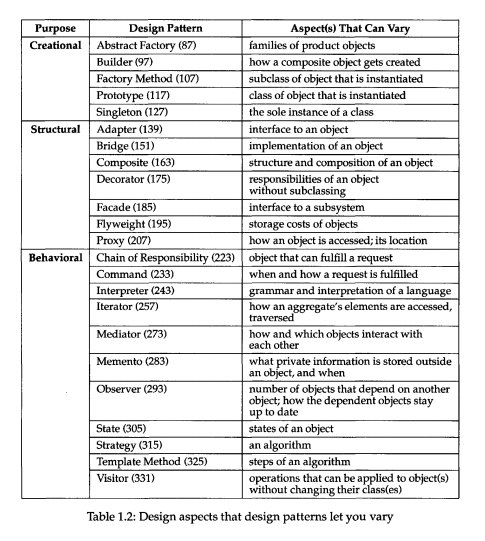
\includegraphics[width=400pt]{design-patterns.png}
\end{figure}

\newpage
\subsection{Creational Patterns}
\subsubsection{Abstract Factory *}
Provide an interface for creating families of related or dependent objects without specifying their concrete classes.

\textbf{Applicability}

Use the Abstract Factory pattern when
\begin{itemize}
    \item a system should be independent of how its products are created, composed, and represented.
    \item a system should be configured with one of multiple families of products.
    \item a family of related product objects is designed to be used together, and you need to enforce this constraint.
    \item you want to provide a class library of products, and you want to reveal just their interfaces, not their implementations.
\end{itemize}

\textbf{Consequences}

The Abstract Factory pattern has the following benefits and liabilities:
\begin{itemize}
    \item It isolates concrete classes.
    \item It makes exchanging product families easy.
    \item It promotes consistency among products.
    \item Supporting new kinds of products is difficult.
\end{itemize}

\begin{figure}[h]
    \centering
    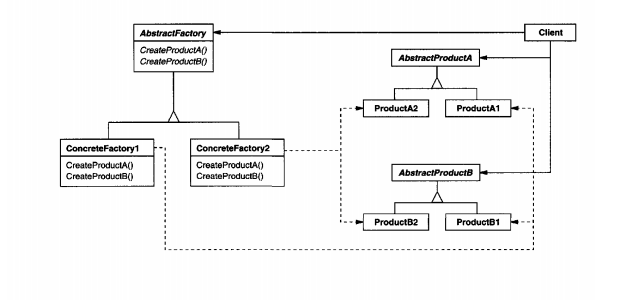
\includegraphics[width=14cm]{diagrams/pattern-1-abstract-factory.png}
\end{figure}

\newpage
\subsubsection{Builder}
Separate the construction of a complex object from its representation so
that the same construction process can create different representations.


\textbf{Applicability}

Use the Builder pattern when
\begin{itemize}
    \item the algorithm for creating a complex object should be independent of the parts that make up the object and how they're assembled.
    \item the construction process must allow different representations for the object that's constructed.
\end{itemize}

\textbf{Consequences}
\begin{itemize}
    \item It lets you vary a product's internal representation.
    \item It isolates code for construction and representation.
    \item It gives you finer control over the construction process.
\end{itemize}

\begin{figure}[h]
    \centering
    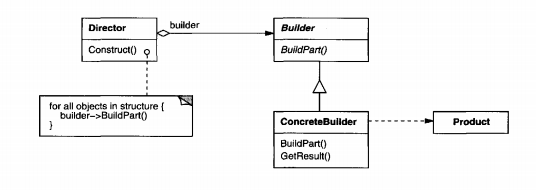
\includegraphics[width=14cm]{diagrams/patterns-2-builder.png}
\end{figure}



\newpage
\subsubsection{Factory Method *}
Define an interface for creating an object, but let subclasses decide which class to instantiate. Factory Method lets a class defer instantiation to subclasses.


\textbf{Applicability}

Use the Factory Method pattern when
\begin{itemize}
    \item a class can't anticipate the class of objects it must create.
    \item a class wants its subclasses to specify the objects it creates.
    \item classes delegate responsibility to one of several helper subclasses, and you want to localize the knowledge of which helper subclass is the delegate.
\end{itemize}

\textbf{Consequences}

Factory methods eliminate the need to bind application-specific classes into your code. The code only deals with the Product interface; therefore it can work with any user-defined ConcreteProduct classes.

A potential disadvantage of factory methods is that clients might have to subclass the Creator class just to create a particular ConcreteProduct object. Subclassing is fine when the client has to subclass the Creator class anyway, but otherwise the client now must deal with another point of evolution.

Factory Method has the additional consequences:
\begin{itemize}
    \item Provides hooks for subclasses.
    \item Connects parallel class hierarchies.
\end{itemize}

\begin{figure}[h]
    \centering
    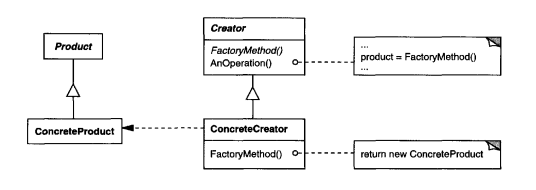
\includegraphics[width=14cm]{diagrams/pattern-3-factory-method.png}
\end{figure}

\newpage
\subsubsection{Prototype}
Specify the kinds of objects to create using a prototypical instance, and create new objects by copying this prototype.

\textbf{Applicability}

Use the Prototype pattern 
\begin{itemize}
    \item when a system should be independent of how its products are created, composed, and represented
    \item when the classes to instantiate are specified at run-time, for example, by dynamic loading.
    \item to avoid building a class hierarchy of factories that parallels the class hierarchy of products.
    \item when instances of a class can have one of only a few different combinations of state.
\end{itemize}

\textbf{Consequences}

Prototype has many of the same consequences that Abstract Factory and Builder have: It hides the concrete product classes from the client, thereby reducing the number of names clients know about. Moreover, these patterns let a client work with application-specific classes without modification.

Additional benefits of the Prototype pattern include
\begin{itemize}
    \item Adding and removing products at run-time.
    \item Specifying new objects by varying values
    \item Specifying new objects by varying structure.
    \item Reduced subclassing.
    \item Configuring an application with classes dynamically.
\end{itemize}

\begin{figure}[h]
    \centering
    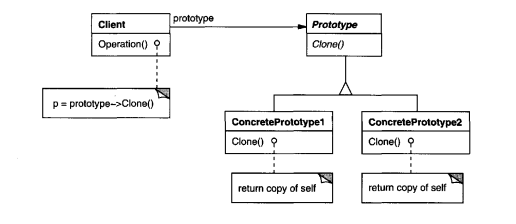
\includegraphics[width=14cm]{diagrams/pattern-4-prototype.png}
\end{figure}

\newpage
\subsubsection{Singleton}
Ensure a class only has one instance, and provide a global point of
access to it.

\textbf{Applicability}

Use the Singleton pattern when
\begin{itemize}
    \item there must be exactly one instance of a class, and it must be accessible to clients from a well-known access point.
    \item when the sole instance should be extensible by subclassing, and clients should be able to use an extended instance without modifying their code.
\end{itemize}

\textbf{Consequences}

The Singleton pattern has several benefits:

\begin{itemize}
    \item Controlled access to sole instance.
    \item Reduced name space.
    \item Permits refinement of operations and representation.
    \item Permits a variable number of instances.
    \item More flexible than class operations.
\end{itemize}

\begin{figure}[h]
    \centering
    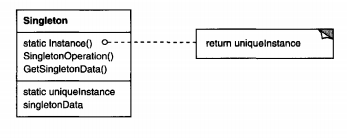
\includegraphics[width=10cm]{diagrams/pattern-5-singleton.png}
\end{figure}


\newpage
\subsection{Structural Patterns}
\subsubsection{Adapter *}
Convert the interface of a class into another interface clients expect. Adapter lets classes work together that couldn't otherwise because of incompatible interfaces.


\textbf{Applicability}

Use the Adapter pattern when
\begin{itemize}
    \item you want to use an existing class, and its interface does not match the one you need.
    \item you want to create a reusable class that cooperates with unrelated or unforeseen classes, that is, classes that don't necessarily have compatible interfaces.
    \item (object adapter only) you need to use several existing subclasses, but it's unpractical to adapt their interface by subclassing every one. An object adapter can adapt the interface of its parent class
\end{itemize}

\textbf{Consequences}

Class and object adapters have different trade-offs. A class adapter

\begin{itemize}
    \item adapts Adaptee to Target by committing to a concrete Adaptee class.
    \item lets Adapter override some ofAdaptee'sbehavior, since Adapter is a subclass of Adaptee.
    \item introduces only one object, no additional pointer indirection is needed for the adaptee
\end{itemize}

An object adapter

\begin{itemize}
    \item lets a single Adapter work with many Adaptees
    \item makes it harder to override Adaptee behavior
\end{itemize}

\begin{figure}[h]
    \centering
    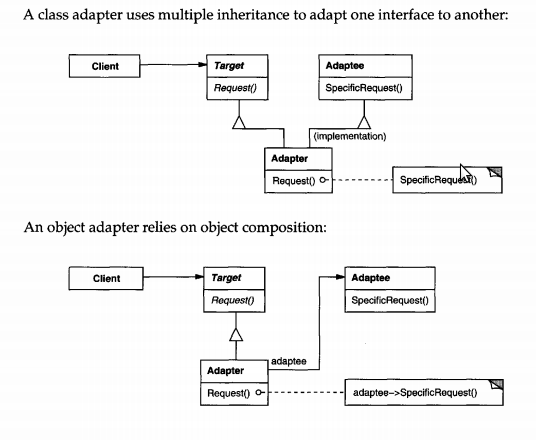
\includegraphics[width=10cm]{diagrams/pattern-6-adapter.png}
\end{figure}

\newpage
\subsubsection{Bridge}
Decouple an abstraction from its implementation so that the two can vary independently.

\textbf{Applicability}

Use the Bridge pattern when

\begin{itemize}
    \item you want to avoid a permanent binding between an abstraction and its implementation. 
    \item both the abstractions and their implementations should be extensible by subclassing.
    \item changes in the implementation of an abstraction should have no impact on clients; that is, their code should not have to be recompiled.
    \item you have a proliferation of hierarchical classes (``nested generalizations")
    \item you want to share an implementation among multiple objects, and this fact should be hidden from the client.
\end{itemize}

\textbf{Consequences}

The Bridge pattern has the following consequences:

\begin{itemize}
    \item Decoupling interface and implementation.
    \item Improved extensibility. 
    \item Hiding implementation details from clients. 
\end{itemize}


\begin{figure}[h]
    \centering
    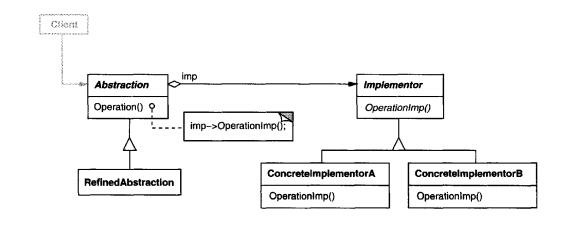
\includegraphics[width=14cm]{diagrams/pattern-7-bridge.png}
\end{figure}

\newpage
\subsubsection{Composite *}
Compose objects into tree structures to represent part-whole hierarchies. Composite lets clients treat individual objects and compositions of objects
uniformly.

\textbf{Applicability}

Use the Composite pattern when
\begin{itemize}
    \item you want to represent part-whole hierarchies of objects.
    \item you want clients to be able to ignore the difference between compositions of objects and individual objects
\end{itemize}

\textbf{Consequences}

The Composite pattern
\begin{itemize}
    \item defines class hierarchies consisting of primitive objects and composite objects
    \item makes the client simple.
    \item makes it easier to add new kinds of components.
    \item can make your design overly general.
\end{itemize}

\begin{figure}[h]
    \centering
    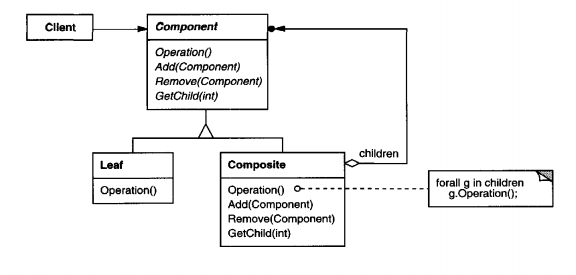
\includegraphics[width=14cm]{diagrams/pattern-8-composite.png}
\end{figure}

\newpage
\subsubsection{Decorator *}
Attach additional responsibilities to an object dynamically. Decorators
provide a flexible alternative to subclassing for extending functionality.

\textbf{Applicability}

Use Decorator
\begin{itemize}
    \item to add responsibilities to individual objects dynamically and transparently, that is, without affecting other objects.
    \item for responsibilities that can be withdrawn.
    \item when extension by subclassing is impractical. 
\end{itemize}

\textbf{Consequences}

The Decorator pattern has at least two key benefits and two liabilities:

\begin{itemize}
    \item More flexibility than static inheritance.
    \item Avoids feature-laden classes high up in the hierarchy.
    \item A decorator and its component aren't identical.
    \item Lots of little objects. 
\end{itemize}

\begin{figure}[h]
    \centering
    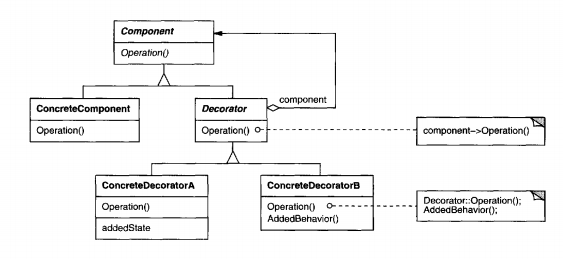
\includegraphics[width=14cm]{diagrams/pattern-9-decorator.png}
\end{figure}

\newpage
\subsubsection{Facade}
Provide a unified interface to a set of interfaces in a subsystem. Facade defines a higher-level interface that makes the subsystem easier to use.

\textbf{Applicability}

Use the Facade pattern when
\begin{itemize}
    \item you want to provide a simple interface to a complex subsystem
    \item there are many dependencies between clients and the implementation classes of an abstraction
    \item you want to layer your subsystems.
\end{itemize}

\textbf{Consequences}

The Facade pattern offers the following benefits:
\begin{itemize}
    \item It shields clients from subsystem components, thereby reducing the number of objects that clients deal with and making the subsystem easier to use.
    \item It promotes weak coupling between the subsystem and its clients.
    \item It doesn't prevent applications from using subsystem classes if they need to. Thus you can choose between ease of use and generality
\end{itemize}

\begin{figure}[h]
    \centering
    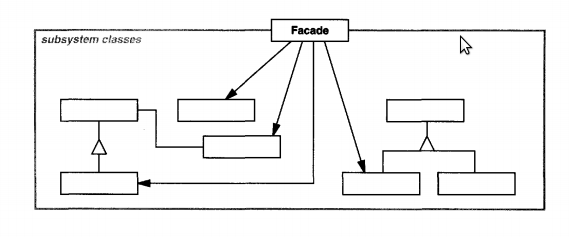
\includegraphics[width=14cm]{diagrams/pattern-10-facade.png}
\end{figure}

\newpage
\subsubsection{Flyweight}
Use sharing to support large numbers of fine-grained objects efficiently.

\textbf{Applicability}

The Flyweight pattern's effectiveness depends heavily on how and where it's
used. Apply the Flyweight pattern when all of the following are true:
\begin{itemize}
    \item An application uses a large number of objects
    \item Storage costs are high because of the sheer quantity of objects.
    \item Most object state can be made extrinsic.
    \item Many groups of objects may be replaced by relatively few shared objects once extrinsic state is removed.
    \item The application doesn't depend on object identity. Since flyweight objects may be shared, identity tests will return true for conceptually distinct objects.
\end{itemize}

\textbf{Consequences}

Flyweights may introduce run-time costs associated with transferring, finding,
and/or computing extrinsic state. However, such costs are offset by space savings, which increase as more flyweights are shared.


\begin{figure}[h]
    \centering
    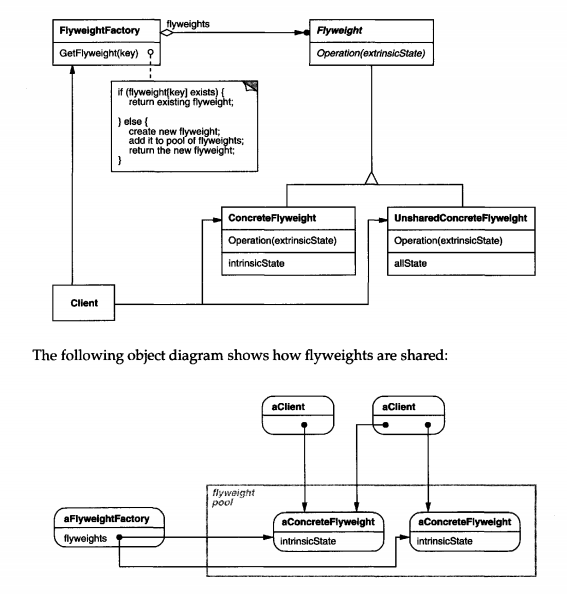
\includegraphics[width=11cm]{diagrams/pattern-11-flyweight.png}
\end{figure}


\newpage
\subsubsection{Proxy}
Provide a surrogate or placeholder for another object to control access to it.

\textbf{Applicability}

Proxy is applicable whenever there is a need for a more versatile or sophisticated reference to an object than a simple pointer. Here are several common situations in which the Proxy pattern is applicable:
\begin{itemize}
    \item A remote proxy provides a local representative for an object in a different address space.
    \item A virtual proxy creates expensive objects on demand.
    \item A protection proxy controls access to the original object. Protection proxies are useful when objects should have different access rights.
    \item A smart reference is a replacement for a bare pointer that performs additional actions when an object is accessed.
\end{itemize}

\textbf{Consequences}

The Proxy pattern introduces a level of indirection when accessing an object. The additional indirection has many uses, depending on the kind of proxy:
\begin{itemize}
    \item A remote proxy can hide the fact that an object resides in a different address space.
    \item A virtual proxy can perform optimizations such as creating an object on demand.
    \item Both protection proxies and smart references allow additional housekeeping tasks when an object is accessed
\end{itemize}

\begin{figure}[h]
    \centering
    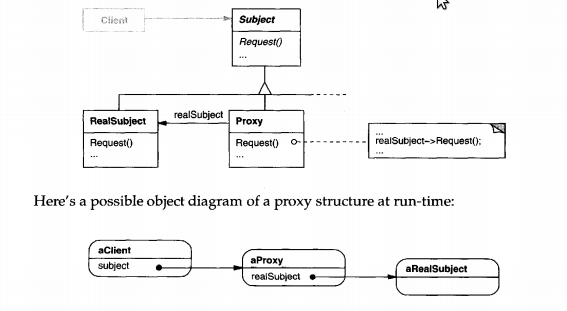
\includegraphics[width=14cm]{diagrams/pattern-12-proxy.png}
\end{figure}

\newpage
\subsection{Behavioural Patterns}
\subsubsection{Chain of Responsibility}
Avoid coupling the sender of a request to its receiver by giving more than one object a chance to handle the request. Chain the receiving objects and pass the request along the chain until an object handles it.

\textbf{Applicability}

Use Chain of Responsibility when

\begin{itemize}
    \item more than one object may handle a request, and the handler isn't known a priori.
    \item you want to issue a request to one ofseveral objects without specifying the receiver explicitly.
    \item the set of objects that can handle a request should be specified dynamically.
\end{itemize}

\textbf{Consequences}

Chain of Responsibility has the following benefits and liabilities:
\begin{itemize}
    \item Reduced coupling.
    \item Added flexibility in assigning responsibilities to objects
    \item Receipt isn't guaranteed.
\end{itemize}

\begin{figure}[h]
    \centering
    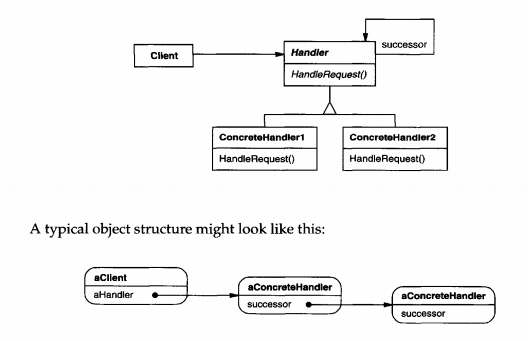
\includegraphics[width=14cm]{diagrams/pattern-13-chain-of-responsibility.png}
\end{figure}

\newpage
\subsubsection{Command}
Encapsulate a request as an object, thereby letting you parameterize clients with different requests, queue or log requests, and support undo-able
operations.

\textbf{Applicability}

Use the Command pattern when you want to

\begin{itemize}
    \item parameterize objects by an action to perform.
    \item specify, queue, and execute requests at different times.
    \item support undo.
    \item support logging changes so that they can be reapplied in case of a system crash.
    \item structure a system around high-level operations built on primitives operations.
\end{itemize}

\textbf{Consequences}

The Command pattern has the following consequences:
\begin{itemize}
    \item Command decouples the object that invokes the operation from the one that knows how to perform it.
    \item Commands are first-class objects. They can be manipulated and extended like any other object.
    \item You can assemble commands into a composite command.
    \item It's easy to add new Commands, because you don't have to change existing classes.
\end{itemize}

\begin{figure}[h]
    \centering
    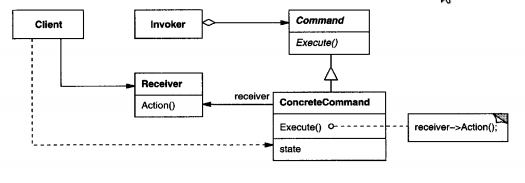
\includegraphics[width=14cm]{diagrams/pattern-14-command.png}
\end{figure}

\newpage
\subsubsection{Interpreter}

Use the Interpreter pattern when there is a language to interpret, and you can represent statements in the language as abstract syntax trees. The Interpreter pattern works best when

\textbf{Applicability}

Use the Command pattern when you want to

\begin{itemize}
    \item the grammar is simple. For complex grammars, the class hierarchy for the grammar becomes large and unmanageable. 
    \item efficiency is not a critical concern. The most efficient interpreters are usually not implemented by interpreting parse trees directly but by first translating them into another form.
\end{itemize}

\textbf{Consequences}

The Interpreter pattern has the following benefits and liabilities:
\begin{itemize}
    \item It's easy to change and extend the grammar
    \item Implementing the grammar is easy.
    \item Complex grammars are hard to maintain.
    \item Easier to add new ways to interpret expressions.
\end{itemize}

\begin{figure}[h]
    \centering
    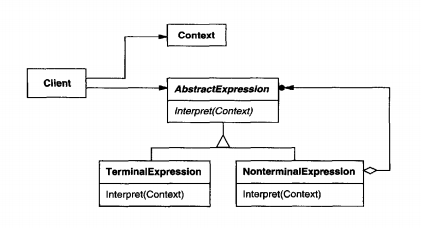
\includegraphics[width=11cm]{diagrams/pattern-15-interpreter.png}
\end{figure}

\newpage
\subsubsection{Iterator}
Provide a way to access the elements of an aggregate object sequentially without exposing its underlying representation.

\textbf{Applicability}

Use the Iterator pattern

\begin{itemize}
    \item to access an aggregate object's contents without exposing its internal representation (i.e. a list).
    \item to support multiple traversals of aggregate objects.
    \item to provide a uniform interface for traversing different aggregate structures (that is, to support polymorphic iteration)
\end{itemize}

\textbf{Consequences}

The Iterator pattern has three important consequences:
\begin{itemize}
    \item It supports variations in the traversal of an aggregate
    \item Iterators simplify the Aggregate interface.
    \item More than one traversal can be pending on an aggregate.
\end{itemize}

\begin{figure}[h]
    \centering
    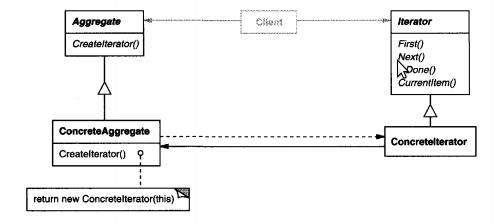
\includegraphics[width=14cm]{diagrams/pattern-16-iterator.png}
\end{figure}

\newpage
\subsubsection{Mediator}
Define an object that encapsulates how a set of objects interact. Mediator promotes loose coupling by keeping objects from referring to each other explicitly, and it lets you vary their interaction independently.

\textbf{Applicability}

Use the Mediator pattern when

\begin{itemize}
    \item a set of objects communicate in well-defined but complex ways.The resulting interdependencies are unstructured and difficult to understand. 
    \item reusing an object is difficult because it refers to and communicates with many other objects.
    \item a behavior that's distributed between several classes should be customizable without a lot of subclassing
\end{itemize}

\textbf{Consequences}

The Mediator pattern has the following benefits and drawbacks:
\begin{itemize}
    \item It limits subclassing.
    \item It decouples colleagues.
    \item It simplifies object protocols.
    \item It abstracts how objects cooperate.
    \item It centralizes control.
\end{itemize}

\begin{figure}[h]
    \centering
    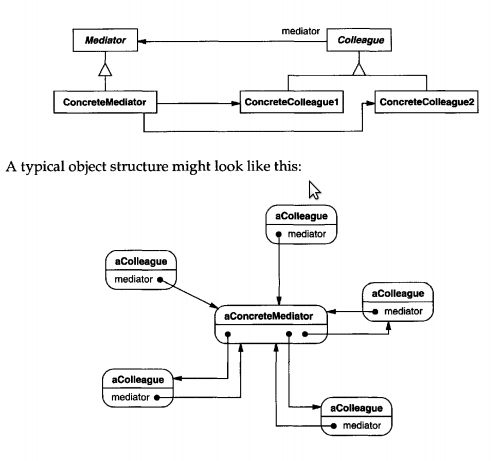
\includegraphics[width=10cm]{diagrams/pattern-17-mediator.png}
\end{figure}

\newpage
\subsubsection{Memento}
Without violating encapsulation, capture and externalize an object's internal state so that the object can be restored to this state later.


\textbf{Applicability}

Use the Memento pattern when

\begin{itemize}
    \item a snapshot of (some portion of) an object's state must be saved so that it can be restored to that state later.
    \item a direct interface to obtaining the state would expose implementation details and break the object's encapsulation.
\end{itemize}

\textbf{Consequences}

The Memento pattern has several consequences:
\begin{itemize}
    \item Preserving encapsulation boundaries.
    \item It simplifies Originator.
    \item Using mementos might be expensive.
    \item Defining narrow and wide interfaces.
    \item Hidden costs in caring for mementos.
\end{itemize}

\begin{figure}[h]
    \centering
    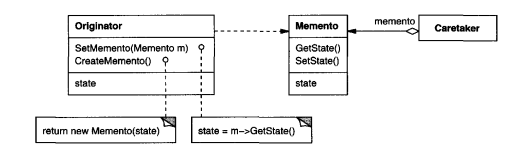
\includegraphics[width=14cm]{diagrams/pattern-18-memento.png}
\end{figure}

\newpage
\subsubsection{Observer *}
Define a one-to-many dependency between objects so that when one object changes state, all its dependents are notified and updated automatically.


\textbf{Applicability}

Use the Observer pattern in any of the following situations:

\begin{itemize}
    \item When an abstraction has two aspects, one dependent on the other. Encapsulating these aspects in separate objects lets you vary and reuse them independently.
    \item When a change to one object requires changing others, and you don't know how many objects need to be changed.
    \item When an object should be able to notify other objects without making assumptions about who these objects are.In other words, you don't want these objects tightly coupled.
\end{itemize}

\textbf{Consequences}

The Observer pattern lets you vary subjects and observers independently. Further benefits and liabilities of the Observer pattern include the following:
\begin{itemize}
    \item Abstract coupling between Subject and Observer.
    \item Support for broadcast communication.
    \item Unexpected updates.
\end{itemize}

\begin{figure}[h]
    \centering
    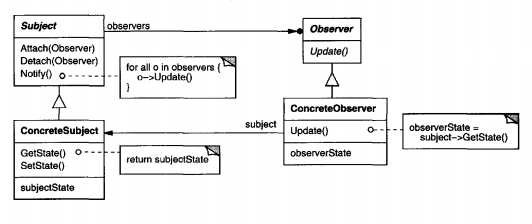
\includegraphics[width=14cm]{diagrams/pattern-19-observer.png}
\end{figure}

\newpage
\subsubsection{State}
Allow an object to alter its behavior when its internal state changes. The object will appear to change its class.

\textbf{Applicability}

Use the State pattern in either of the following cases:

\begin{itemize}
    \item An object's behavior depends on its state, and it must change its behavior at run-time depending on that state. 
    \item Operations have large, multipart conditional statements that depend on the object's state. 
\end{itemize}

\textbf{Consequences}

The State pattern has the following consequences:
\begin{itemize}
    \item It localizes state-specific behavior and partitions behavior for different states.
    \item It makes state transitions explicit.
    \item State objects can be shared.
\end{itemize}

\begin{figure}[h]
    \centering
    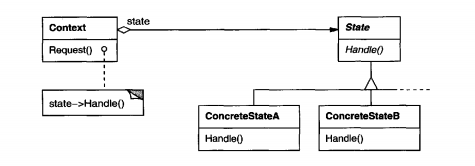
\includegraphics[width=14cm]{diagrams/pattern-20-state.png}
\end{figure}

\newpage
\subsubsection{Strategy *}
Define a family of algorithms, encapsulate each one, and make them
interchangeable. Strategy lets the algorithm vary independently from clients that use it.

\textbf{Applicability}

Use the Strategy pattern when

\begin{itemize}
    \item many related classes differ only in their behavior. Strategies provide a way to configure a class with one of many behaviors. 
    \item you need different variants of an algorithm. 
    \item an algorithm uses data that clients shouldn't know about.
    \item a class defines many behaviors, and these appear as multiple conditional statements in its operations.
\end{itemize}

\textbf{Consequences}

The Strategy pattern has the following benefits and drawbacks:
\begin{itemize}
    \item Families of related algorithms.
    \item An alternative to subclassing.
    \item Strategies eliminate conditional statements. 
    \item A choice of implementations. 
    \item Clients must be aware of different Strategies.
    \item Communication overhead between Strategy and Context.
    \item Increased number of objects.
\end{itemize}

\begin{figure}[h]
    \centering
    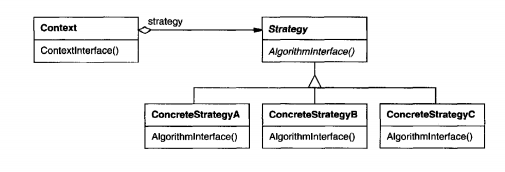
\includegraphics[width=14cm]{diagrams/pattern-21-strategy.png}
\end{figure}

\newpage
\subsubsection{Template Method *}
Define the skeleton of an algorithm in an operation, deferring some steps to subclasses. Template Method lets subclasses redefine certain steps of an algorithm without changing the algorithm's structure.

\textbf{Applicability}

The Template Method pattern should be used

\begin{itemize}
    \item to implement the invariant parts of an algorithm once and leave it up to subclasses to implement the behavior that can vary.
    \item when common behavior among subclasses should be factored and localized in a common class to avoid code duplication.
    \item to control subclasses extensions.
\end{itemize}

\textbf{Consequences}

Template methods are a fundamental technique for code reuse. Template methods lead to an inverted control structure. This refers to how a parent class calls the operations of a subclass and not the other way around.

Template methods call the following kinds of operations:
\begin{itemize}
    \item concrete operations (either on the ConcreteClass or on client classes)
    \item concrete AbstractClass operations (i.e., operations that are generally useful to subclasses)
    \item primitive operations (i.e., abstract operations)
    \item factory methods
    \item hook operations, which provide default behavior that subclasses can extend if necessary. A hook operation often does nothing by default.
\end{itemize}

\begin{figure}[h]
    \centering
    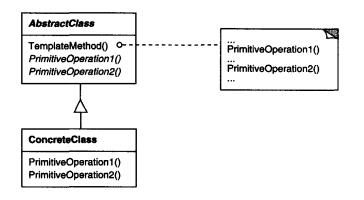
\includegraphics[width=10cm]{diagrams/pattern-22-template.png}
\end{figure}


\newpage
\subsubsection{Visitor}
Represent an operation to be performed on the elements of an object structure. Visitor lets you define a new operation without changing the classes of the elements on which it operates.

\textbf{Applicability}

Use the Visitor pattern when

\begin{itemize}
    \item an object structure contains many classes of objects with differing interfaces, and you want to perform operations on these objects that depend on their concrete classes.
    \item  many distinct and unrelated operations need to be performed on objects in an object structure, and you want to avoid ``polluting" their classes with these operations.
    \item the classes defining the object structure rarely change, but you often want to define new operations over the structure.
\end{itemize}

\textbf{Consequences}

Some of the benefits and liabilities of the Visitor pattern are as follows:
\begin{itemize}
    \item Visitor makes adding new operations easy.
    \item A visitor gathers related operations and separates unrelated ones.
    \item Adding new ConcreteElement classes is hard.
    \item Visiting across class hierarchies.
\end{itemize}

\begin{figure}[h]
    \centering
    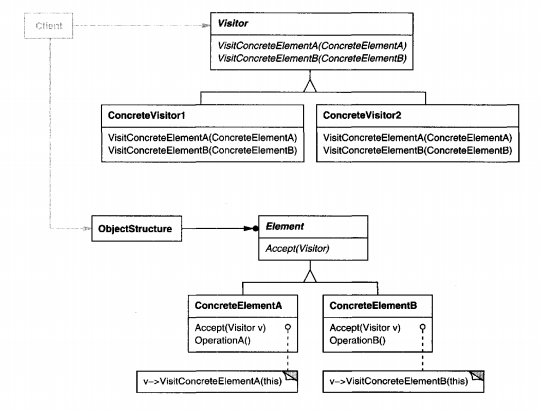
\includegraphics[width=11cm]{diagrams/pattern-23-visitor.png}
\end{figure}

\begin{thebibliography}{}
\bibitem{}
Gamma, E., Helm, R., Johnson, R.,, Vlissides, J. M. (1994). Design Patterns: Elements of Reusable Object-Oriented Software. Addison-Wesley Professional. ISBN: 0201633612

\end{thebibliography}
\end{document}
